\documentclass[10pt]{article}
\usepackage[margin=.65in]{geometry}\usepackage{amsmath,tikz,hyperref}
\setlength{\parindent}{0pt}\setlength{\parskip}{6pt}
\begin{document}
\textbf{Computed scale, trimming and divisor storage}\hfill2026-10-31\\T-1174. Producer proof; independent source-fidelity review pending.

The checked small-power computation supplies a nonzero canonical scale and its decoded equality $s=a^m$. The complete word transform followed by terminal-zero trimming and zero padding represents
\[
 T_m(f)=a^{-m}f(aX+b).
\]
The source-model theorem no longer requires a separately supplied scale-equality premise.
\begin{center}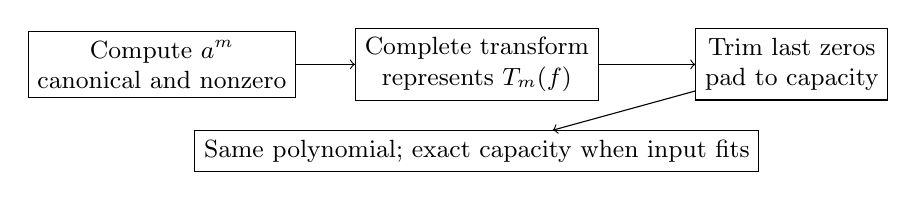
\begin{tikzpicture}[every node/.style={draw,align=center,font=\small}]
\node(a)at(0,0){Compute $a^m$\\canonical and nonzero};
\node(b)at(4,0){Complete transform\\represents $T_m(f)$};
\node(c)at(8,0){Trim last zeros\\pad to capacity};
\node(d)at(4,-1.1){Same polynomial; exact capacity when input fits};
\draw[->](a)--(b);\draw[->](b)--(c);\draw[->](c)--(d);
\end{tikzpicture}\end{center}
The word theorem assumes prime $1<p<2^{31}$, canonical coefficients and parameters, nonzero $a$, length $\le6$ and $m\in\{0,\ldots,5\}$. The list polynomial laws require only a commutative ring.

The trim model tests whether the last word is zero, then removes it. Polynomial preservation holds for any fuel. Fuel at least the original length suffices to finish with no terminal zero. Padding appends zeros and preserves the polynomial. Exact capacity requires the original length to fit; oversized inputs are not silently truncated.

The array/list coefficient bridge connects these storage laws to the previously decoded transform. Source divisor capacities are 3 for $u$ and 2 for $v$. Composition with the divisor degree/domain and Mumford-validity theorem remains next. This is a logical model of scale, last/pop and zero-initialized prefix copying, not compiled-Rust equivalence or geometric class transport.

Seventeen main declarations and fifteen controls passed, with 32 named standard-axiom readbacks. Controls include empty/all-zero lists, internal/trailing zeros, insufficient fuel, capacities 2/3, over-capacity exclusion, and powers 0/2/3. Modulo 17, separate representation examples give
\[
 [1,2,1]\xrightarrow{a=2,b=3,m=2}[4,4,1],\qquad
 [5,0]\xrightarrow{a=2,b=3,m=3}[7,0]
\]
after trimming and padding. These are not a claim that the two examples form a valid divisor on a named curve.

Scale, controls and readback passed first attempt. Trim attempt 1 needed the dropLast-length rewrite and an available empty-list lemma; attempt 2 passed. Bridge attempt 1 contained notation parsed as an initial-segment token; attempt 2 passed after spacing correction. All failures and nonfatal warnings remain recorded. Final readback contains only standard axioms.

Sources: \texttt{projective\_law\_gate.rs} transform/map\_divisor; prior small-power and polynomial proofs; pinned Mathlib last-element identity; \href{https://lean-lang.org/doc/api/Init/Data/List/TakeDrop.html}{Lean take/drop semantics}. Existing compiled dependencies remain in the trust boundary. No scientific campaign, timing or cost ratio.
\end{document}
